\documentclass[a4paper,10pt]{article}
\usepackage[utf8]{inputenc}
\usepackage{geometry}
\geometry{
a4paper,
total={170mm,257mm},
left=20mm,
top=20mm,
}
\setlength{\parindent}{0pt}
\usepackage{color}
\newcommand*{\red}{\textcolor{red}}
\usepackage{booktabs}
\usepackage{tabularx}
\usepackage[pdftex]{graphicx}
\usepackage{subcaption}

%opening
\title{Notes on the code}
\author{Steven Court}

\begin{document}


\maketitle



\section{Agent based simulation: CIPRO\_LBgrowth.cpp}
This program is based on code written by Bartek and simulates his evolutionary experiments as precisely as possible: individual cells replicate, die, mutate and swim in a chain 
of 3-dimensional, connected wells. The C++ code can be found in the directory ``Agent based simulation/Main program'' and is compiled
to an executable with the command ``g++ -O3 CIPRO\_LBgrowth.cpp -o run.exe''. To run the code we must supply some terminal parameters, these being the directory into which
the data will be saved, the number of experiments to simulate and a random number seed. For instance: ``./run.exe data 1 7'' will simulate 1 experiment using a random seed
of 7 and store all data into a directory called data.



\subsection{Data produced}
Doing so will produce the following files.
\begin{itemize}
 \item parameters.txt records all parameter values used in the simulation.
 \item nwell.dat stores the populations of each well at set times throughout the simulation; ODs.dat stores the ``optical density'' as measured 
 experimentally (down a 1 mm$^2$ column in the centre of each well).
 \item antibiotic.dat records the antibiotic concentration in each of the wells.
 \item The directory sequenceFiles/ contains all observed evolutionary trajectories, in every well, at the end of every experiment ran.
 The structure of each file is ``x m$_1$ m$_2$ m$_3$'' where the first number x is the number of cells that have followed the evolutionary trajectory
 given by the following numbers: mutation m$_1$, followed by m$_2$, followed by m$_3$ (i.e.~a time ordered list of mutations from which one can construct
 all intermediate genotypes). 
 Since the strain fitness and MIC data taken from Ref.~\ref{} considers the 5 mutations most associated with ciprofloxacin resistance
 the values of m$_i$ are 0 to 4 and there can be at most 5 of them.
 \item The directory strainFiles/ contains separate files for every well of every experiment storing the final abundances (second column) of all 32 strains (labelled
 with integer 0--31) in first column. The strains are numbered in the order they appear in Marcusson2009 \cite{} Table 1 with strains 29--31 being the 3 ommitted in this paper.
 \emph{Should change this so that we label them as actual genomes, ``10100'' for example.}
 \item The directory wellFiles/ contains files storing the final abundance of each mutation for every well of each experiment. 
 The first column is the rank, the second column is the genomic position of the mutation (we currently only have 5 since the modified code ignores passenger mutations)
 and the third column is the abundance of this mutation in the population.
 \item positions\_n\_n.dat stores the (x,y,z)-coord of all cells at the end of an experiment.
\end{itemize}



\subsection{Model parameters}
\begin{itemize}
 \item nwells: number of wells (experiments contain 24 connected wells).
 \item w, h: width and height of the w$\times$w$\times$h~mm$^3$ wells. Values fixed through calibration.
 \item hole\_width, hole\_depth: dimensions of channels connecting the wells. Values fixed through calibration.
 \item max\_no\_drivers: maximum number of driver mutations (since we are now using the data of Marcusson \cite{} and ignore passenger mutations this must
 be set to 5).
 \item diff: bacterial diffusion constant. Around 1.5~mm$^2$/h for E.~coli.
 \item max\_growth\_rate: redundant parameter since experimental growth data is now used. Leave this as 1.0/h.
 \item tmax: experimental time to simulate (in hours).
 \item init\_bact: initial bacteria (randomly distributed throughout first well).
 \item K: carrying capacity of each well.
 \item uni\_antibiotic, max\_antibiotic: determine the antibiotic concentration in well $i$ through: 
 $a_i = \rm{uni\_antibiotic} + \rm{max\_antibiotic}^{(i+1/\rm{nwells})}$.
 \item gamma: the average number of mutations acquired per replication. Currently set to $10^{-3}$ since the genome size of E.~coli
 is on the order of $10^6$ while the basepair mutation probability per replication event is $10^{-9}$.
 \item p\_g$i$: mutation probabilities for each of the 5 driver mutations. $i=0$ to 4 corresponds to the genes
 gyrA1, gyrA2, parC, marR and acrR respectively. p\_g0 is used to match the expected number of mutations per well between
 the simulation and experiment if using smaller population sizes. For instance, in Bartek's experiements with a carrying
 capacity of about $10^8$ and a basepair mutation probability of $10^{-9}$ we expect on average 0.1 gyrA1 mutations per well. Thus,
 if simulating the system using $K=10^5$, and with gamma=$10^{-3}$, we have $10^5\times10^{-3}$ mutations per well and so must 
 have a probability of p\_g0$=10^{-3}$ to ensure an expected value of 0.1 gyrA1 mutations per well.
 The marR and acrR probabilities are suspected to be higher than the others since they can arise from many different mutations. They are currently set to be 10 times higher.\\
 \item X, Y and max\_increase: parameters of an arbitrary function controlling how gamma changes with increasing ciprofloxacin
 concentration $a$; $\gamma(a) = \gamma(0) \left[ 1 + (Xa/\rm{MIC_{WT}})^Y \right]$ until max\_increase, the maximal factor by which the
 mutation rate can increase, is reached.
\end{itemize}



\subsection{Other versions of the code}


\subsubsection{Ciprofloxacin-dependent motility}
Testing the effect of this I had used 2 different implementations, both of which assumed a step function dependence: below some cutoff antibiotic concentration cells
are fully motile, while above this cutoff they are completely immotile. Version (1) used gene-dependent cutoffs, so that the presence of each driver mutation dictated
the cutoff and (2) assumed the cutoff was only dependent on the MIC of a strain with the cutoff being some arbitrary fraction of the MIC. 
We decided the latter was more biologically plausible and also allowed nonmotile cells
to continue reproducing (thus consuming nutrient / contributing to the carrying capacity) but that they could not produce mutant offspring. This was in an attempt
to capture the possible affect of filamentation in the experiment.
The program {\bf CIPRO\_motility\_noMutation.cpp} can be used to simulate version (2) and is in the directory ``Agent based simulation/Cipro-dependent motility''. The parameter
motilityCutoff is the fraction of a strain's MIC above which motility and mutation are disallowed.


\subsubsection{Bartek's original code}
The original unmodified program, 3d\_wells\_phyl\_accumulation.cpp can be found in the directory ``Unmodified program''.
It does not use Bartek's experimental growth data, does not consider specific mutations and their effect on fitness or MIC 
(only distinguishing between passenger and driver mutations) and produces some different data.
Was used to investigate generally how passenger mutations accummulate throughout an experiment.






\subsection{Things to improve}
This code and it's modifications were used to test many things and was always minimally modified from previous versions. As such, I never took the time to
rewrite it for efficiency as for my purposes it wasn't necessary, but there are obvious changes that should be made to make it more efficient. 
For instance, when determining the fitness and MIC of a selected cell, I check all combinations of mutations to determine which strain the cell is
(and thus do it twice); growth() and death\_during\_rep() methods.
It would make more sense to attribute a fitness and MIC field to each cell and only modify this whenever a mutation event occurs.
Since we are no longer considering passenger mutations we do not even need to store a list of mutated sites but could just define a probability table
for each genotype transition. 



 
%%%%%%%%%%%%%%%%%%%%%%%%%%%%%%%%%%%%%%%%%%%%%%%%%%%%%%%%%%%%%%%%%%%%%%%%%%%%%%%%%%%%%%%%%%%%%%%%%%%%%%%%%%%%%
%%%%%%%%%%%%%%%%%%%%%%%%%%%%%%%%%%%%%%%%%%%%%%%%%%%%%%%%%%%%%%%%%%%%%%%%%%%%%%%%%%%%%%%%%%%%%%%%%%%%%%%%%%%%%


 
 
\section{Fisher waves}
As well as simulating the Fisher waves with the full, agent-based simulation we studied them using the set of coupled ODEs corresponding to the discrete Fisher equation
and tau-leaping algorithm. Both of these programs {\bf ODEs\_Euler\_notMixed.java} and {\bf TauLeaping\_nonMixedLB.java} can be found in the ``Other code'' directory.
The size and number of timesteps are hardcoded into the programs. 







 
%%%%%%%%%%%%%%%%%%%%%%%%%%%%%%%%%%%%%%%%%%%%%%%%%%%%%%%%%%%%%%%%%%%%%%%%%%%%%%%%%%%%%%%%%%%%%%%%%%%%%%%%%%%%%
%%%%%%%%%%%%%%%%%%%%%%%%%%%%%%%%%%%%%%%%%%%%%%%%%%%%%%%%%%%%%%%%%%%%%%%%%%%%%%%%%%%%%%%%%%%%%%%%%%%%%%%%%%%%%

 
 \clearpage
 \newpage
 

\section{Data analysis scripts}
The scripts used to produce the figures can be found in the directory ``Data analysis scripts''.
Section \ref{sec:Ex} gives a concrete example of how to apply them to a sample data set and explains their output.

\begin{itemize}
 \item {\bf construct\_mutational\_graph\_ALL\_WELLS.py} is used to generate a weighted mutation graph from the data of multiple experiments. To run it, we must specify
 the path to the directory containing the sequence data from all experiments: ``python construct\_mutational\_graph\_ALL\_WELLS.py path/sequenceFiles''. It calls the 
 script ``construct\_mutational\_graph.py'' and constructs a weighted mutational graph for each individual well.
 If using linux, you can create a gif using these images via the command: ``convert -delay 25 \$(ls -v *.png) filename.gif''.
 This script requires the open source graph vizualisation software Graphviz (automatically present on the school of physics' Linux desktops).
 \item {\bf get\_cumProb\_trajectories\_well\_x.py} plots the cumulative probability of evolutionary trajectories versus their rank for cells in a given well across \emph{all}
 experiments. 
 That is, it calculates the probability that a random cell in the specified well, across all experiments, follows a certain evolutionary trajectory. 
 It uses the data in the sequenceFiles directory and requires this 
 and the desired well to be specified: ``python get\_cumProb\_trajectories\_well\_x.py path/sequenceFiles 23'' will make the cumulative probability plot using the sequence data
 of all cells found in well 23 at the end of all experiments.
 You can make the same plot but only considering cells of a given genotype by using {\bf python get\_cumProb\_trajectories\_well\_x\_endGenotype\_g.py} and supplying the genotype,
 in the form ``11000'', as an extra terminal input. (The order of genes is gyrA1, gyrA2, parC, marR, acrR; values 1 or 0 indicate whether that mutation is present or not).  
 \item {\bf get\_reachedFinalWell.py} will use the sequence files to check how many experiments reached the final well. Must supply path to sequenceFiles directory.
 \item {\bf plot\_driver\_occurrences.py} will plot, for each individual experiment, the 5 mutations against well number indicating in which wells each gene is above some threshold abundance.
 Setting the parameter CUTOFF to 0.1 corresponds to a 10\% experimental detection limit. Set the parameter ``num\_experiments'' to produce the plots for a specified 
 number of experiments, not necessarily hundreds of plots. To run, we must specify the path to the wellFiles directory: ``python plot\_driver\_occurrences.py path/wellFiles''
 and images will be saved in this directory.
 \item {\bf plot\_driver\_probabilities.py} is used to produce a plot that uses the data from all experiments, showing the probability that each mutated gene is present in each
 well above some cutoff. You need to set the number of experiments you wish to average this from by hand in the script and similar to above: 
 ``python plot\_driver\_probabilities.py path/wellFiles''.
 \item {\bf plot\_strain\_occurrences.py} generates plots for individual experiments showing the abundance of each mutated strain across all wells.
 Uses the data found in strainFiles directory: ``python plot\_strain\_occurrences.py path/strainFiles/''.
 Set the desired number of experiments to plot in the code. 
 \item {\bf plot\_strain\_probabilities.py} averages the data from all experiments in the strainFiles directory to produce a plot showing the probability that each strain
 is observed in a given well. Set the number of experiments to average over in the code and run as before: ``python plot\_strain\_probabilities.py path/strainFiles/''.
 %%
 %% FISHER WAVE SCRIPTS
 \item {\bf plot\_fisher\_speed.py} requires the well population data, nwell.dat, from a \emph{single} experiment to calculate the speed of the travelling wave and produce 2 plots.
 The first is of the progression of the wavefront in time and the other contains snapshots of the wave at various points in the experiment (how many points to display is
 controlled by the parameter time\_gap in the script and may need to be modified).
 A similar script {\bf plot\_fisher\_speed\_ANTIBIOTIC.py} makes the same 2 plots but on the fisher wave plot adds a curve showing the antibiotic concentration
 in each well along with the MIC of the wildtype. This requires a concentration data file, antibiotic.dat, to be supplied as a second terminal input. 
 Additionally, {\bf plot\_fisher\_speed\_DENSITY.py} performs the same function but for nwell.dat files containing well densities rather than absolute cell numbers.
 \item {\bf get\_mean\_speed.py} takes an nwell.dat file containing multiple experiments and calculates the mean speed and standard deviation.
 \item {\bf make\_wave\_profile.py} reads in nwell.dat for a single experiment to produce the wave profile data to be plotted in order to compare
 the profiles between simulation and experiment.
 It calculates the speed of the wave $v$ and then collapses the profiles from various timepoints onto the comoving coordinate $z=x-vt$. 
 make\_wave\_profile\_DENSITIY.py is the same but for density data rather than absolute numbers.
\end{itemize}


\subsection{Other scripts}
Some other scripts that may be useful are:

\begin{itemize}
 \item {\bf make\_fitness\_landscape\_allWells.py} creates plots of ``true fitness'' vs strain along with the mutational graph for each well. The proxy used for 
 true fitness of a given strain is $f(1-P_d)$ where $f$ is the fitness of the strain relative to the wildtype in the absence of antibiotic and $P_d$ is the probability
 of death upon replication due to the antibiotic, $a$, and strain's MIC: $P_d = (a/\rm{MIC})^2$. 
 To run, the path to the directory containing the antibiotic profile, antibiotic.dat, file must be given: ``python make\_fitness\_landscape\_allWells.py path''.
 The command ``convert -delay 25 \$(ls -v *.png) file.gif'' will convert the generated images into a gif in order to see how the strain viabilities change across a given experiment.
\end{itemize}


 

 
%%%%%%%%%%%%%%%%%%%%%%%%%%%%%%%%%%%%%%%%%%%%%%%%%%%%%%%%%%%%%%%%%%%%%%%%%%%%%%%%%%%%%%%%%%%%%%%%%%%%%%%%%%%%%
%%%%%%%%%%%%%%%%%%%%%%%%%%%%%%%%%%%%%%%%%%%%%%%%%%%%%%%%%%%%%%%%%%%%%%%%%%%%%%%%%%%%%%%%%%%%%%%%%%%%%%%%%%%%%
 
 
 \clearpage
 \newpage
 
 
\section{Tau-leaping implementation} 
I have also written an alternative simulation of Bartek's system which was motivated by the idea of performing some sort of Monte Carlo parameter
fitting to experimental data, thus requiring much faster simulation times. The Tau-leaping algorithm does not track individual cells but is an
efficient approximation to the Gillespie algorithm. The basic program, as well as a trial of it being used in a MC-fitting can be found in the directory 
``TauLeaping''. The program is written in JAVA and all .java files can be simultaneously compiled with the command ``javac *.java'' and the program is run,
for example, using ``java TauLeapSystem'' (and may require some terminal inputs).
The experimentally determined growth data, strain fitnesses and MICs from the literature \cite{} are read in from the input files growthData\_LB\_nonMixed.dat, 
Fitnesses.dat and MICs.dat respectively.\\

{\bf TauLeap\_MCopt\_diff\_FOOD\_Channels.java} was used to attempt a parameter fitting between the time-series of each well. 
The parameters being fitted here were the diffusion constants across each connecting channel and the stochastic simulation was matched to
``TEST\_DATA'', produced from the deterministic system of ODEs. (Note that this code was written as a test of proof of principle and is not very general. 
Currently the comparison is between population time-series of all wells, made at specific points in time. The TEST\_DATA file was produced with a 
fixed timestep of 0.001~h so if altering this in the tau-leaping simulation, TEST\_DATA should be reproduced with the correct timestep, or the comparison
method altered to account for this).

To test the basic procedure an initial set of parameter values is chosen, some distance measure between the deterministic data and stochastic simulation
is calculated, parameters are modified in some manner, if new distance is less than the previous distance we accept the parameter change, if not, we
accept it with some probability. (See Results and Discussion notes for more details).\\

Note also that this program now explicitly includes nutrient (or food) molecules. This was reintroduced since initially, rather than attributing a diffusion
parameter to each \emph{channel} I attributed it to each \emph{well}. Thus the left and rightwards rates through given channel were different, leading to some wells
acting as sinks. Since the growth rate was limited only by the density in a well, if one well was very quickly losing cells to a neighbouring sink, many more birth events
could take place than the well's carrying capacity.\\

The program where diffusion parameters are asigned to wells is {\bf TauLeap\_MCopt\_diff\_FOOD\_Wells.java}.\\


 

 
 
 
 
 
 



 
 \clearpage
 \newpage
 
\section{Calibration / other}
There have been many intermediate versions of the code, and many side programs written to test various aspects of the system. Here I do not list them all but
only the ones which may be useful in the future. They can be found in the directory Other\_code.
 
\begin{itemize}
 \item {\bf diff\_3d\_linux.cpp} was used to calibrate the dimensions of the wells and connecting channels. It solves the diffusion equation in a chain of connected
 3-dimensional wells and produced data to be compared to Bartek's experiments with methyl blue and with the stochastic simulations containing diffusing
 but non-reproducing bacteria.
 \item {\bf explicit\_nutrient\_diffusion.cpp} was used to model food molecules and their diffusion explicitly in order to check the effect on the growth curve. 
 Bacteria are only able to consume molecules within a defined local volume,
 and we were checking to see if this allowed the growth curve with non-mixed LB medium to be reproduced using the growth function obtained from the well-mixed experiments.
 \item {\bf coupled\_bacteria\_nutrient.nb} is a mathematica notebook solving the coupled PDEs of a nutrient and bacterial density field. It was also used to test the effect 
 on the growth curve when explicitly modelling the nutrient and its diffusion.
\end{itemize}
 
 

 
 
 
 
 
 
 
 
 
 
 
 
 \clearpage
 \newpage
 
\section{An example of a simulation and analysis}\label{sec:Ex}
So as to be clear on how to run a simulation, use the analysis scripts and intepret the output, here I describe the process in full and explain the figures produced.
The data for this system is in the SampleData directory so you can reproduce these plots if you want to familiarise yourself with the scripts.
The simulation was ran 100 times with a maximum ciprofloxacin concentration of 1000 ng/ml and all other parameters can be found in parameters.txt.
Copy and paste the analysis scripts into the SampleData directory and run the following commands.\\


 
-- ``python get\_reachedFinalWell.py max1000/sequencesFiles/''.\\
Will print to terminal that 100 out of 100 experiments reached the final well.\\

-- ``python construct\_mutational\_graph\_ALL\_WELLS.py max1000/sequencesFiles/''.\\
Will print out a weighted mutational graph for every well, which can be combined to a form a gif. Figure \ref{fig:mutGraph} shows such a plot for one well.\\

-- ``python get\_cumProb\_trajectories\_well\_x.py max1000/sequencesFiles/ 23''.\\
Plots the cumulative probability vs rank of all trajectories followed by cells in well 23, from the 100 experiments (Figure \ref{fig:cumProb}).\\

-- ``python plot\_driver\_occurrences.py max1000/wellFiles/''.\\
Plots the probability that each \emph{mutation} is above some defined cutoff abundance in each well for every individual experiment.
Figure \ref{fig:driverOccurence} shows an example experiment.\\

-- ``python plot\_driver\_probabilities.py max1000/wellFiles/''.\\
Figure \ref{fig:driverProbability}

-- ``python plot\_strain\_occurrences.py max1000/strainFiles/''.\\
Plots the abundances of each \emph{strain} across all wells (one plot for every individual experiment).
Figure \ref{fig:strainOccurence} shows an example experiment, that corresponding to Fig.~\ref{fig:driverOccurence}.\\

-- ``python plot\_strain\_probabilities.py max1000/strainFiles/''.\\
Figure \ref{fig:strainProbability}

-- ``python make\_fitness\_landscape\_allWells.py max1000/''.\\
Produces a plot of ``true fitness'' of all strains, along with the mutational graph, for every well. Combine these into a gif to see how fitness changes
across an experiment. (It will also produce the same information but in the form of a histogram; these aren't as pretty).\\

With respect to the fisher wave plots, since this data set was produced using an exponential ciprofloxacin gradient, we should not expect
to see a constant speed wavefront or well defined wave profiles. However, for the sake of using these scripts, nwell\_exp1.dat contains the
well population data from the first experiment (copy and pasted from nwell.dat) and we can run:\\

-- ``python plot\_fisher\_speed.py nwell\_exp1.dat''.\\
Produces 2 plots, Figs.~\ref{fig:waveprofiles} and \ref{fig:waveprofiles} showing progression of the wavefront and snapshots of the population at various times.\\

-- ``python make\_wave\_profile.py nwell\_exp1.dat''.\\
Will print out the data for the collapsed waveforms, that is the comoving coordinate $z=x-vt$. You can plot this data however you want and compare it
to Bartek's experimental wave data or his transformed growth curves.\\



 
 \clearpage
 \newpage


 
\begin{figure}
  \centering
  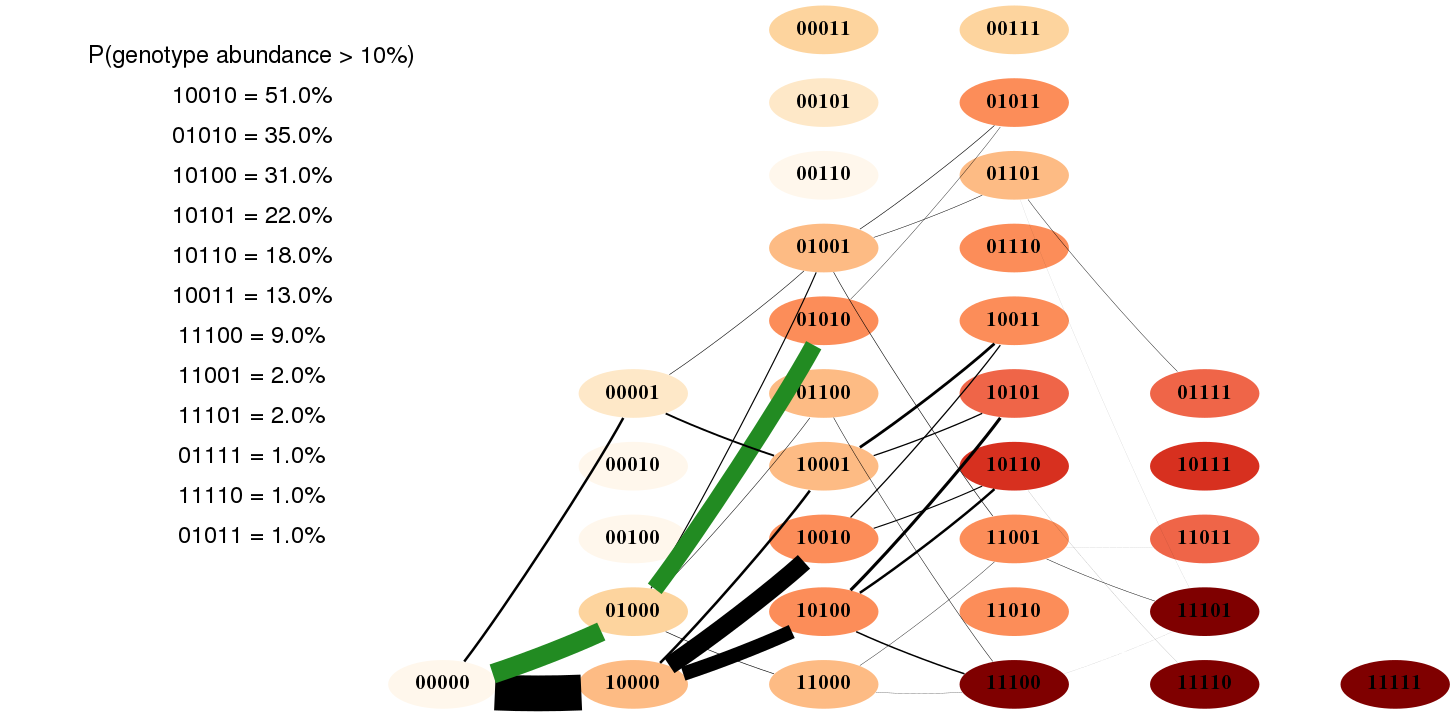
\includegraphics[width=0.95\linewidth]{MutGraph_23}
\caption{The weighted mutational graph of well 23, obtained from analysing the evolutionary trajectories of all cells found in this well
across 100 experiments. Each node is a genotype, with 0s and 1s representing the absence or presence of the mutations gyrA1, gyrA2, parC, marR and acrR.
The node colours correspond to the logarithm of the strain's MICs, with darker colours corresponding to higher MIC values. The edges (mutations) are weighted
as follows: every evolutionary trajectory from all cells found in well 23 from all experiments is read in, and all mutations are counted. Each specific mutation is then
weighted as a proportion of the total number of mutations. It may be the case that to get these figures looking pretty you have to play with the weighting
parameter ``ARBITRARY\_SCALING'' (make it larger if you want all edges to be thicker). The trajectory coloured in green corresponds to the single trajectory
that was followed by the greatest number of cells across all experiments. The values on the left hand side of the graph correspond to the probability that a given
genotype has an abundance $>$10\% in an experiment. That is, from the first number we can say that taking a single experiment, there is a 51\% chance that strain
10010 is present in well 23 with an abundance of $>$10\% (i.e.~it was in 51 out of the 100 simulations we ran). Notice that this genotype does not correspond
to the end-point of the most followed trajectory (green path). This may seem confusing at first but is ok: it just means that although the strain 10010 is most likely to
be present above 10\%, it is also more likely to have produced mutant offspring whoes evolutionary trajectories obviously do not end here. That is, an absolute greater number 
of cells may have passed through the pathway to 10010 than through the green path, but I have defined evolutionary trajectries using there endpoints. 
Maybe there is a better thing to plot here? We see that there are a number of viable strains in the final well (1000~ng/ml) and many possible pathways.}
\label{fig:mutGraph}
\end{figure}

 
 
 
 \begin{figure}
  \centering
  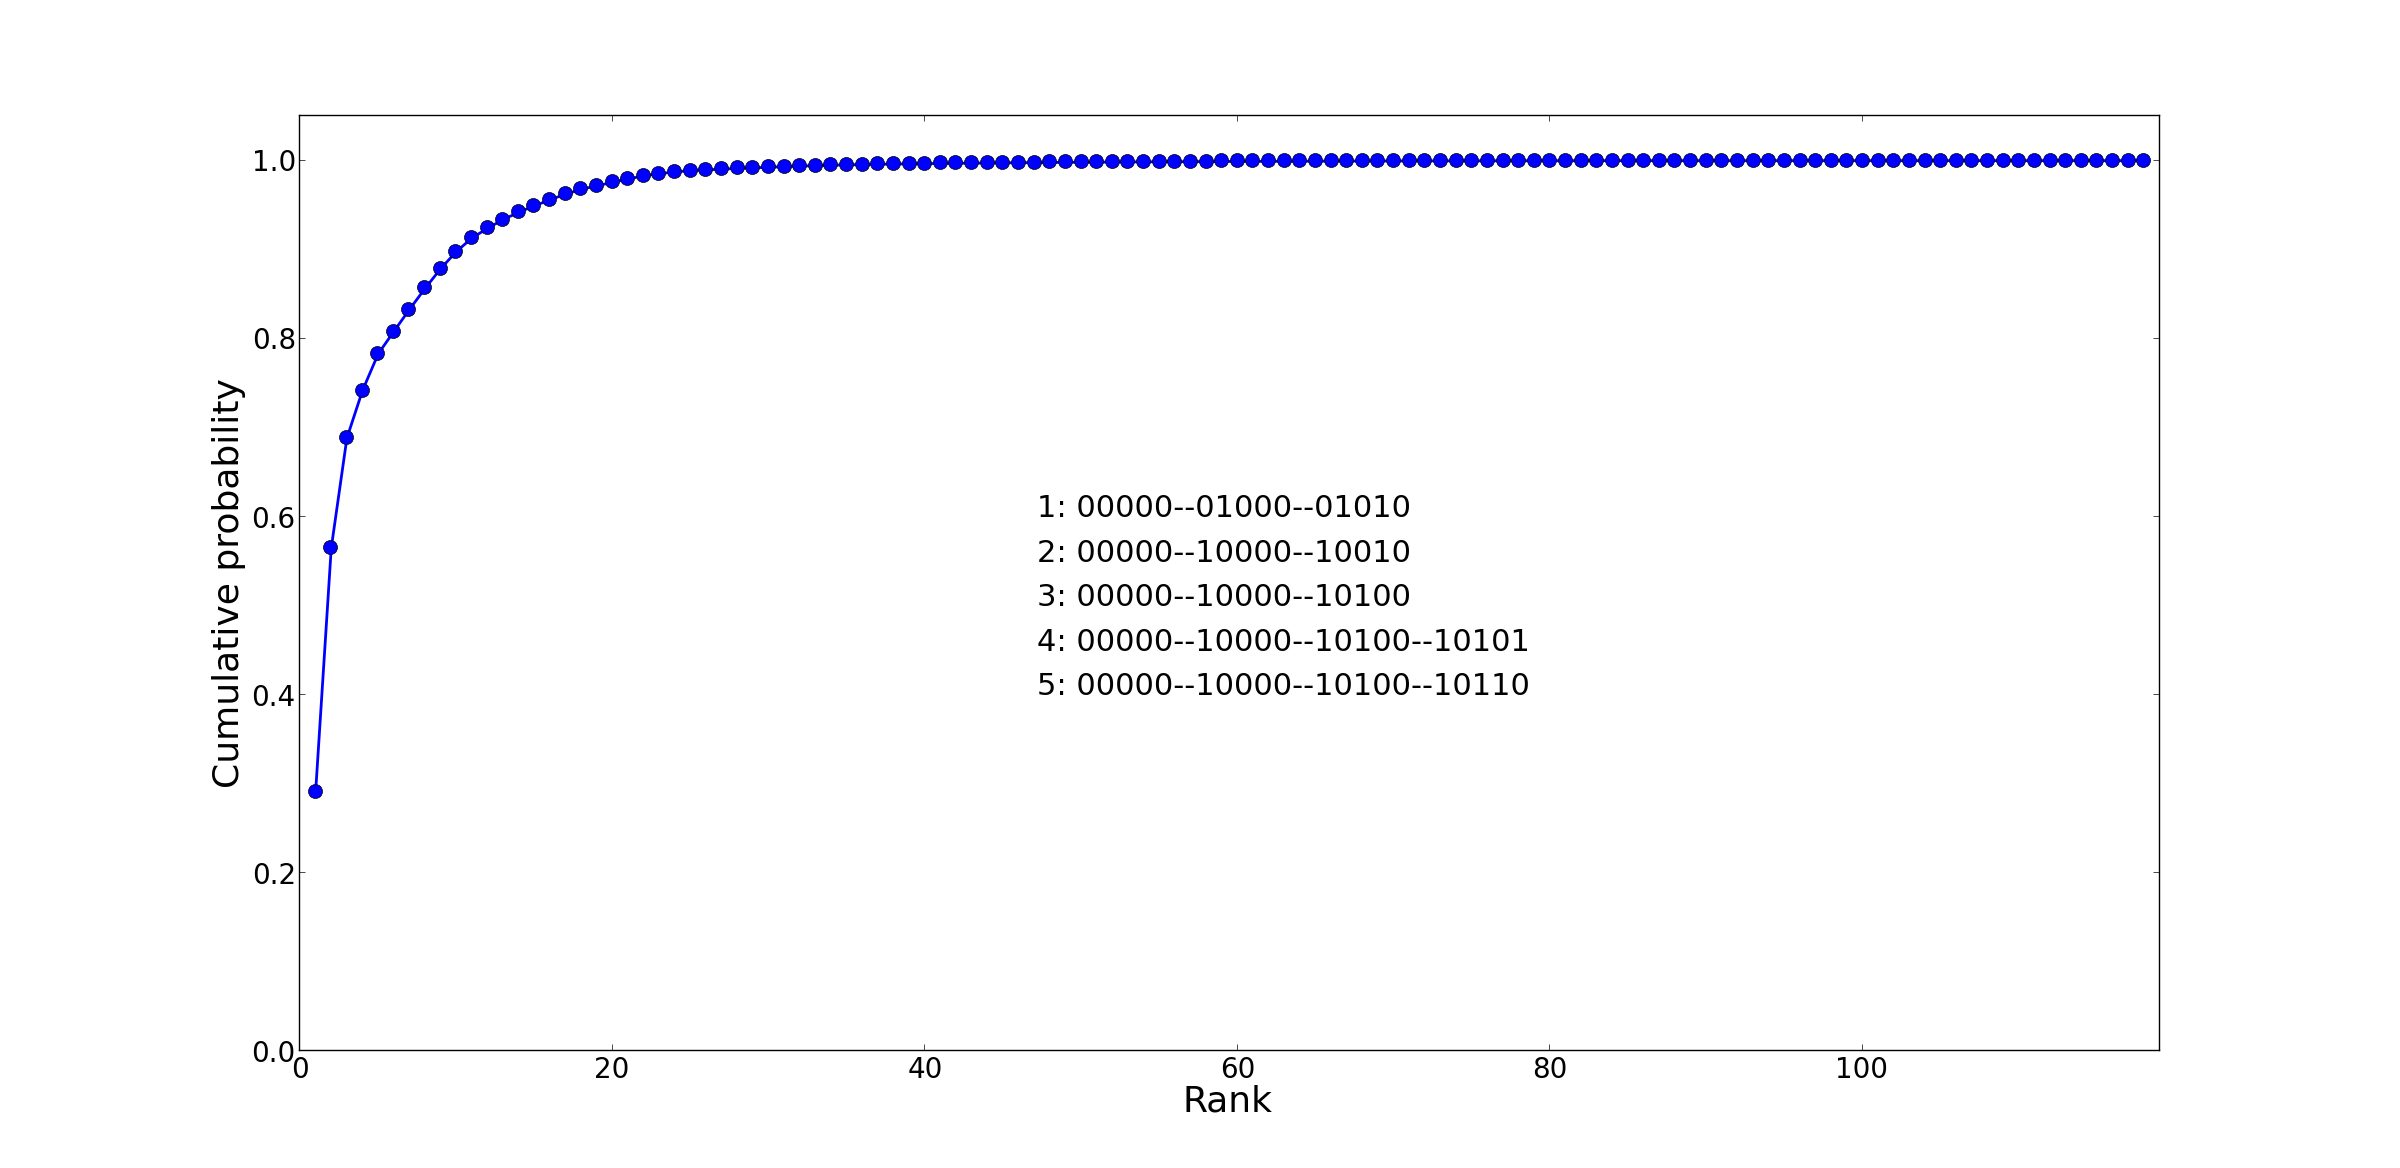
\includegraphics[width=0.95\linewidth]{trajectories_cumProb}
\caption{The cumulative probability vs rank of all evolutionary trajectories followed by cells found in well 23 from all 100 experiments.
The text inset defines the 5 most probable (i.e.~number 1 corresponds to the green trajectory above).
Although a huge number of trajectories are plotted here, it is likely that many of these will result from a small number of cells that may not actually
be viable in the final well, but that have just happened to migrate there and not died by the end of the experiment.
Interestingly, despite having a very large number of trajectories and viable endpoints, we see that the 5 most followed trajectories
account for 80\% of all trajectories.}
\label{fig:cumProb}
\end{figure}

 
 
  \begin{figure}
  \centering
  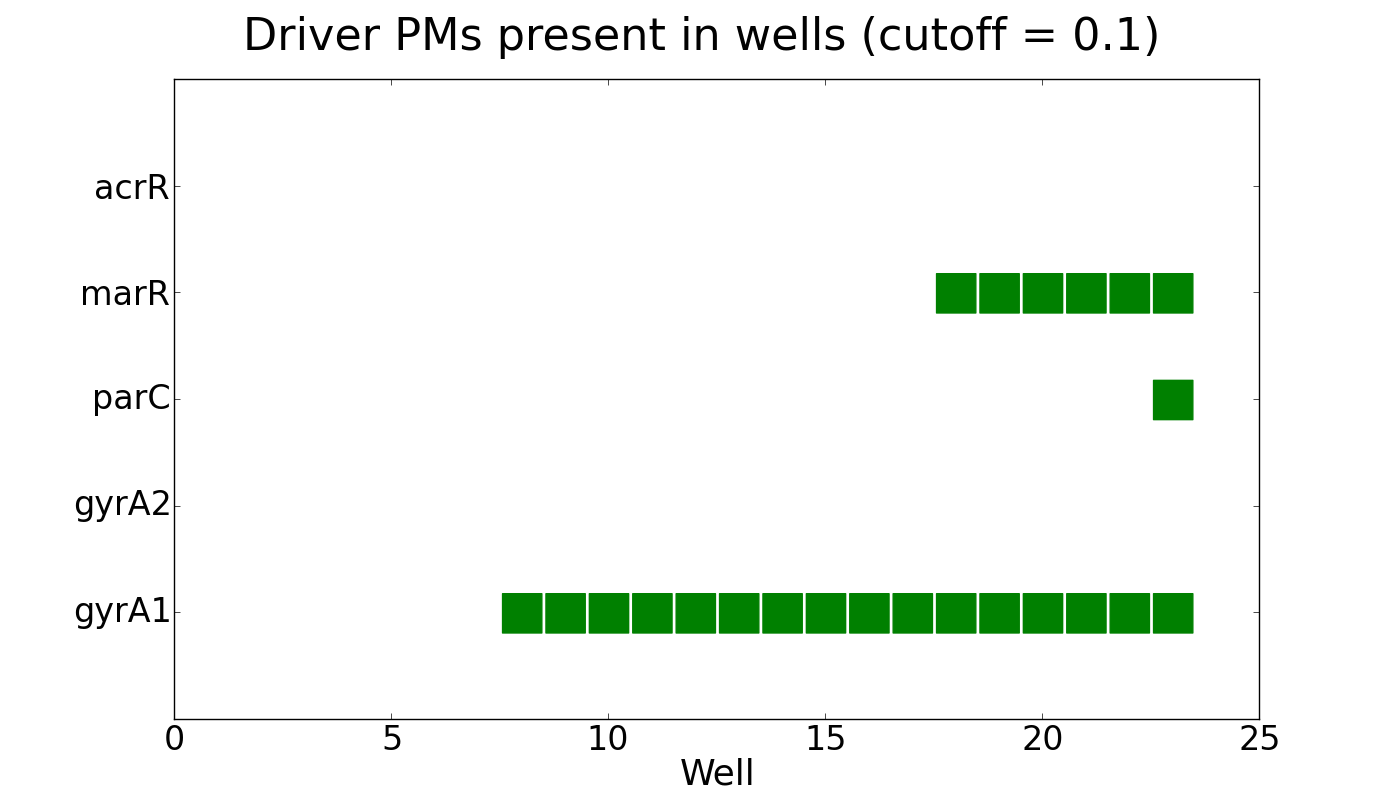
\includegraphics[width=0.95\linewidth]{Experiment_0_cutoff_0p1}
\caption{Gene detection in a single experiment. This plot corresponds to the first of the 100 experiments ran and shows at which well each gene has an
abundance higher than the experimental detectability threshold (defined as 10\%). We can see that in this experiment gyrA2 and acrR are never detectable.
The script that produced this can produce the same plot for all 100 expeirments (set this parameter in the script) which is a useful way to see by eye
the large variability between experiments.}
\label{fig:driverOccurrence}
\end{figure}


 \begin{figure}
  \centering
  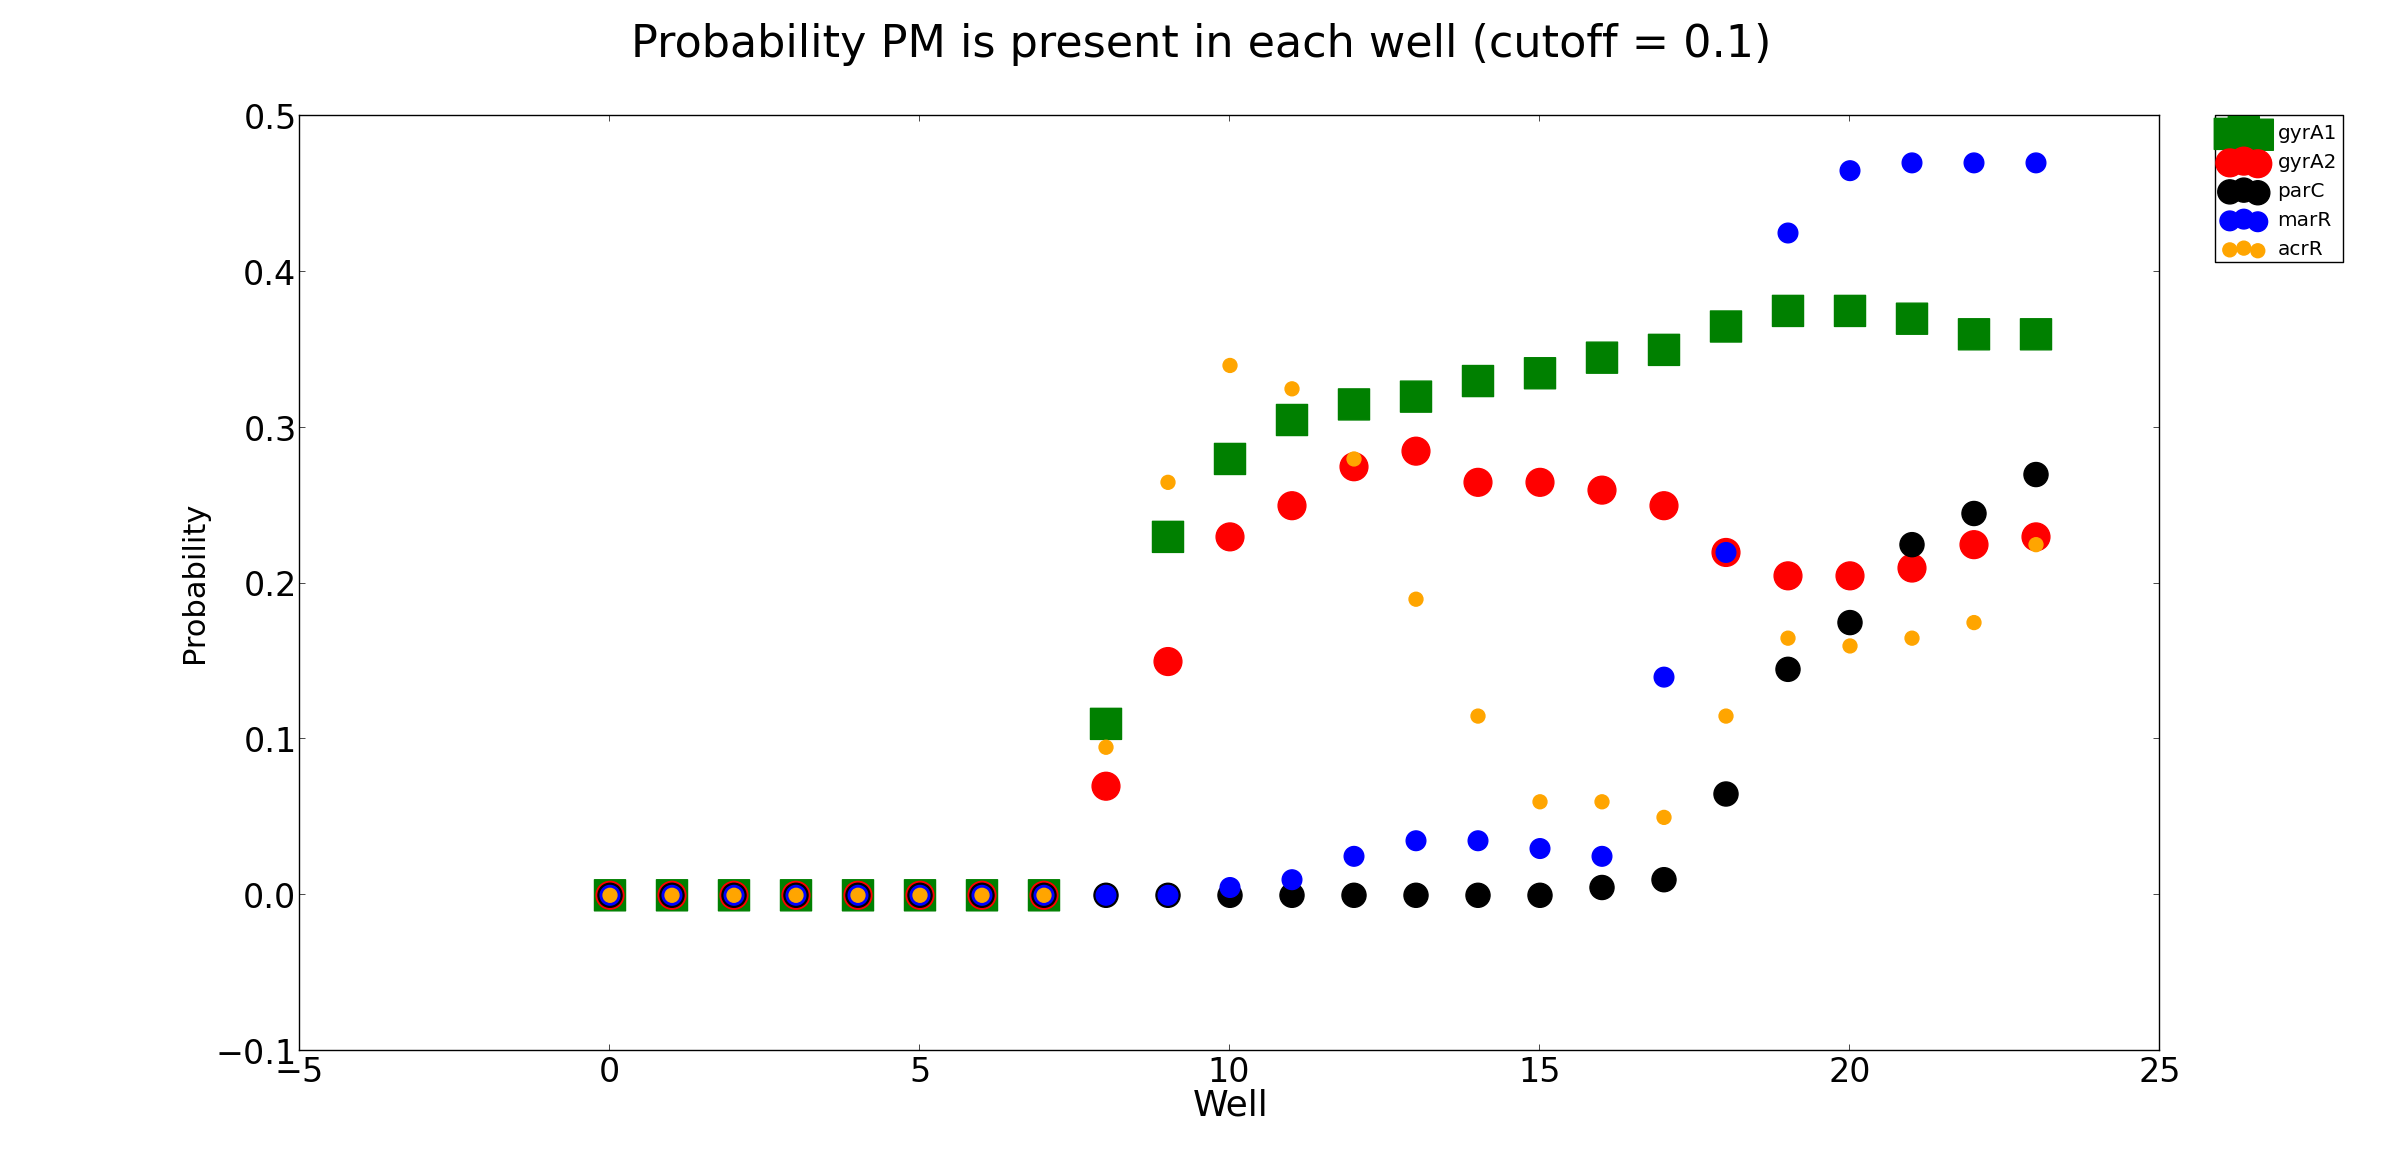
\includegraphics[width=0.95\linewidth]{gene_probabilities}
\caption{The probability, calculated from all 100 experiments, that each gene is detectable in a given well at the end of the experiment.
For this set of parameters and a maximum ciprofloxacin concentration of 1000~ng/ml, we find that no mutated gene is ever detectable until well 8.
This could be useful for informing Bartek's DNA sequencing and in testing for extra effects such as an MIC-dependent motility which would force
mutations to accummulate in earlier wells.
These plots are tricky to interpret and contain interesting non-monotonicities due to the complicated genotype-MIC-fitness relations.}
\label{fig:driverProbability}
\end{figure}



  \begin{figure}
  \centering
  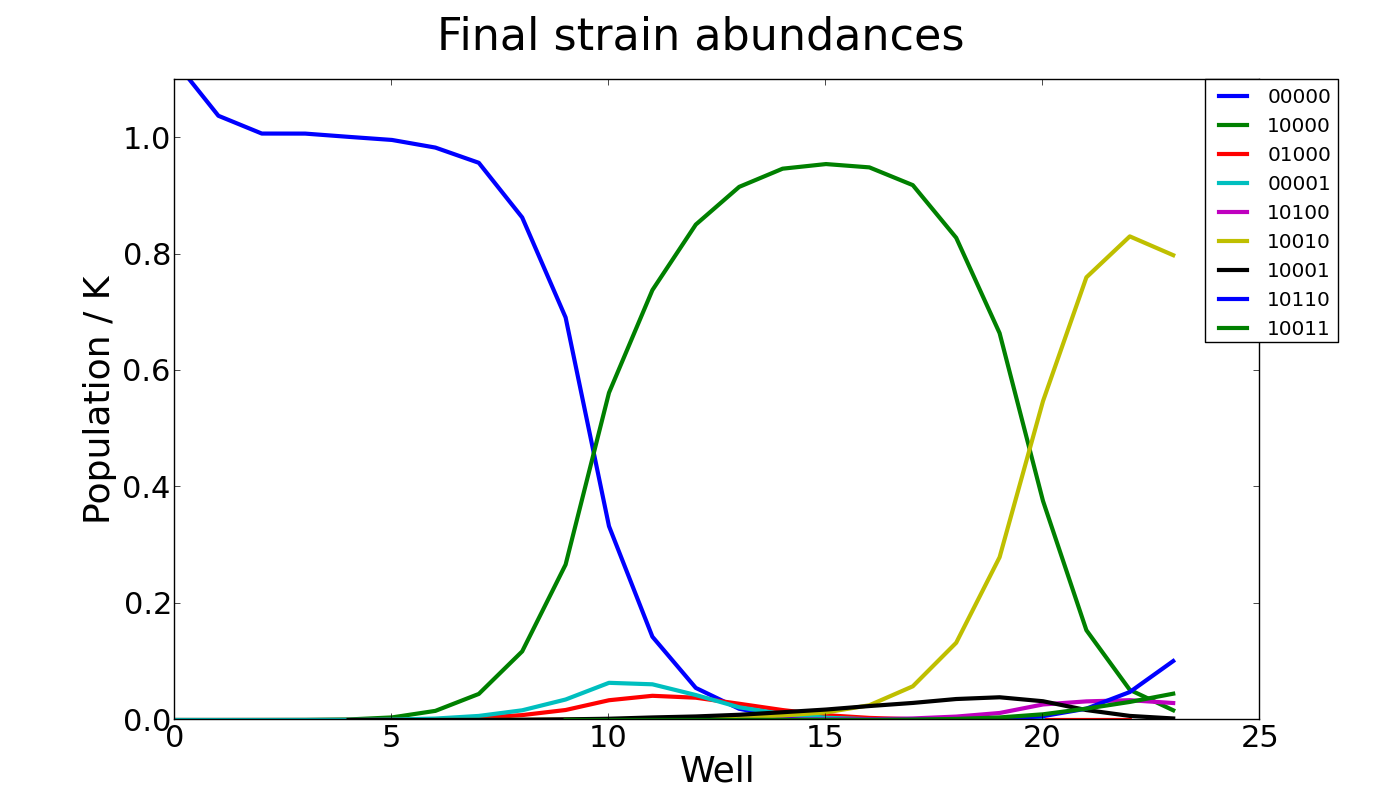
\includegraphics[width=0.95\linewidth]{Strains_Experiment_0}
\caption{The progression of strains through a single experiment (the first, as in Fig.~\ref{fig:driverOccurrence}). We see 2 events in which
mutated genes rise close to fixation; gyrA1 around well 10 and marR around well 20. These plots wre interesting but probably not of much practical use
since Bartek cannot get this information easily/cheaply from his experiments.}
\label{fig:strainOccurrence}
\end{figure}




 \begin{figure}
  \centering
  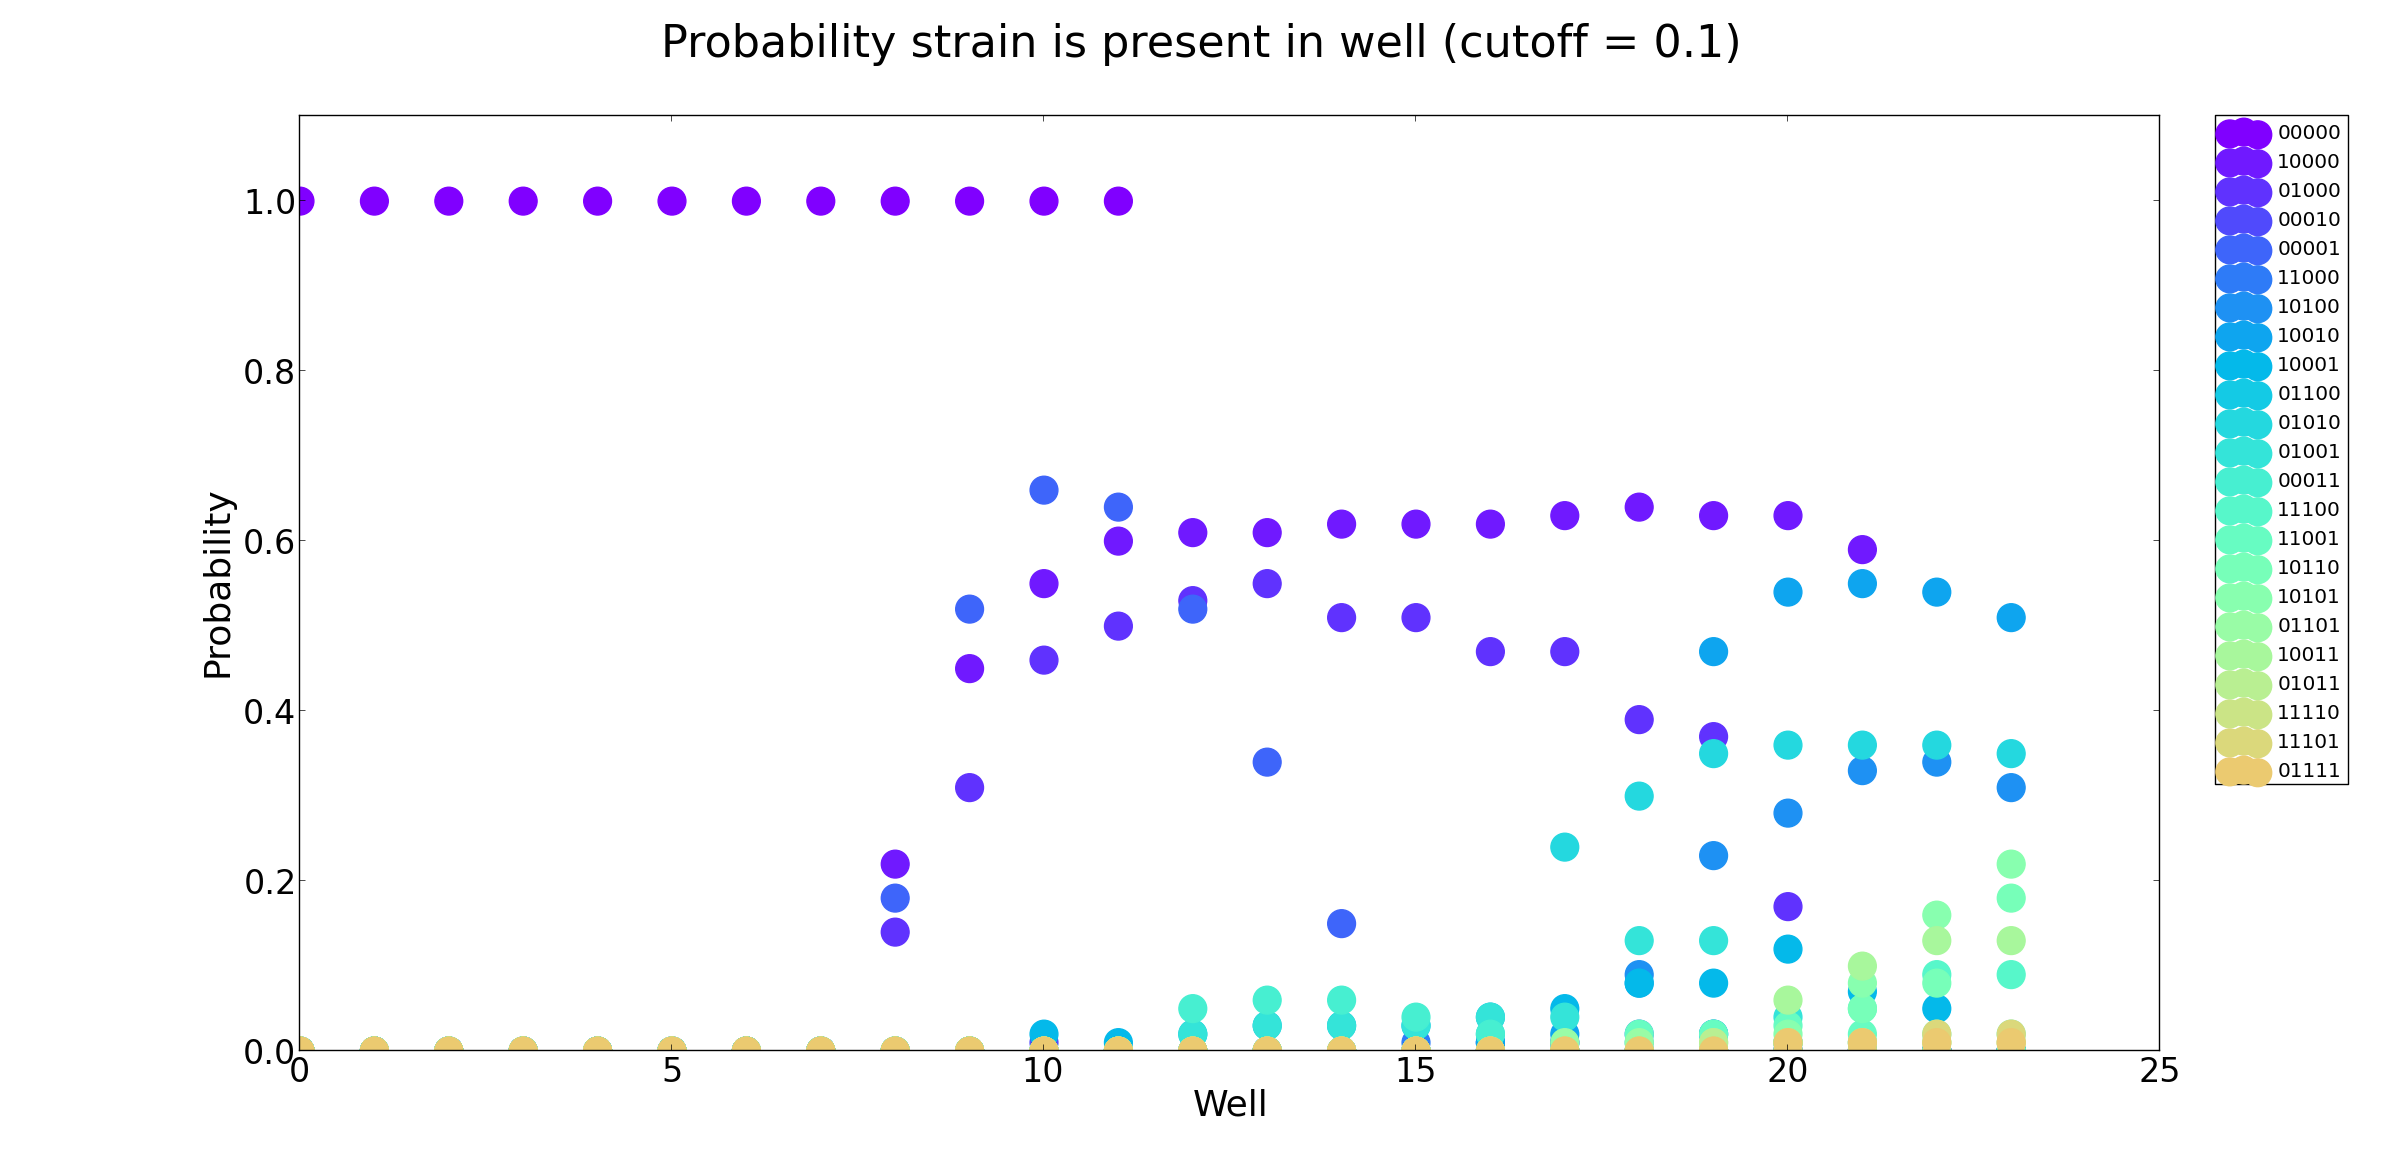
\includegraphics[width=0.95\linewidth]{strain_probabilities}
\caption{The probability that given strains are above an abundance of 10\% in each well, calculated from all 100 experiments.
Such plots are complicated to interpret and again are likely not practically useful since Bartek cannot determine this information.}
\label{fig:strainProbabilities}
\end{figure}
 
 
 
  \begin{figure}
  \centering
  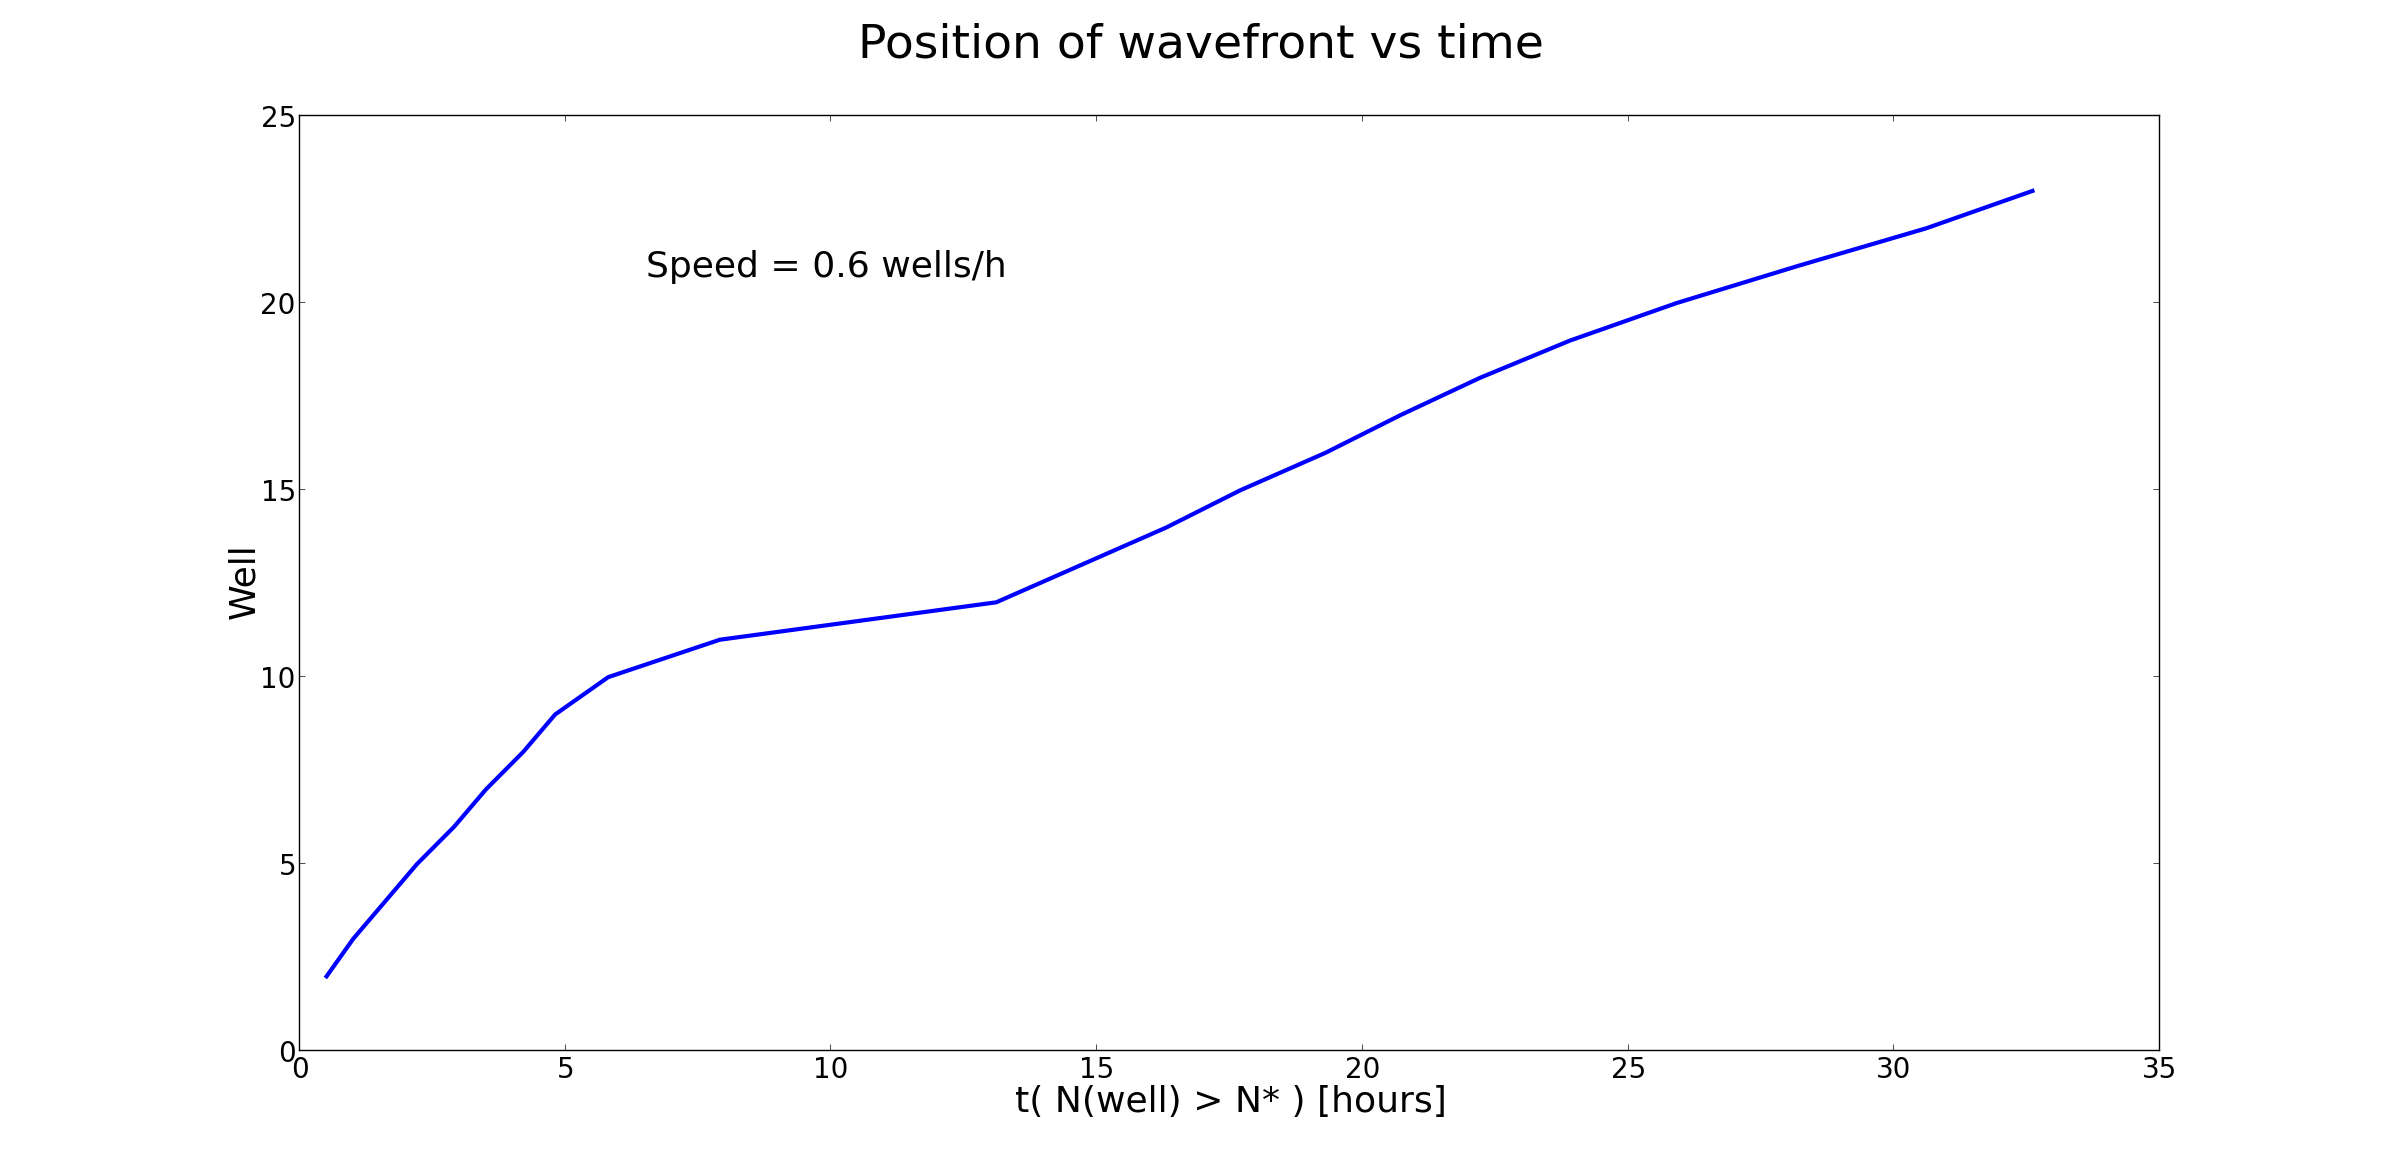
\includegraphics[width=0.95\linewidth]{wavefront}
\caption{The progression of the wavefront in time. Since this simulation was in the presence of ciprofloxacin we do not expect to see a true travelling wave.
(Without antibiotic we would see a straight line, whos gradient could be read off as the wavespeed. The stated speed of 0.6 wells/h is thus not
an accurate or sensible measure in this example.)
We can see that the progress of the wave slows dramatically around well 10 until some beneficial mutation occurs and a secondary
``wave'' with a different speed commences.}
\label{fig:wavefront}
\end{figure}
 
 
 
 
  \begin{figure}
  \centering
  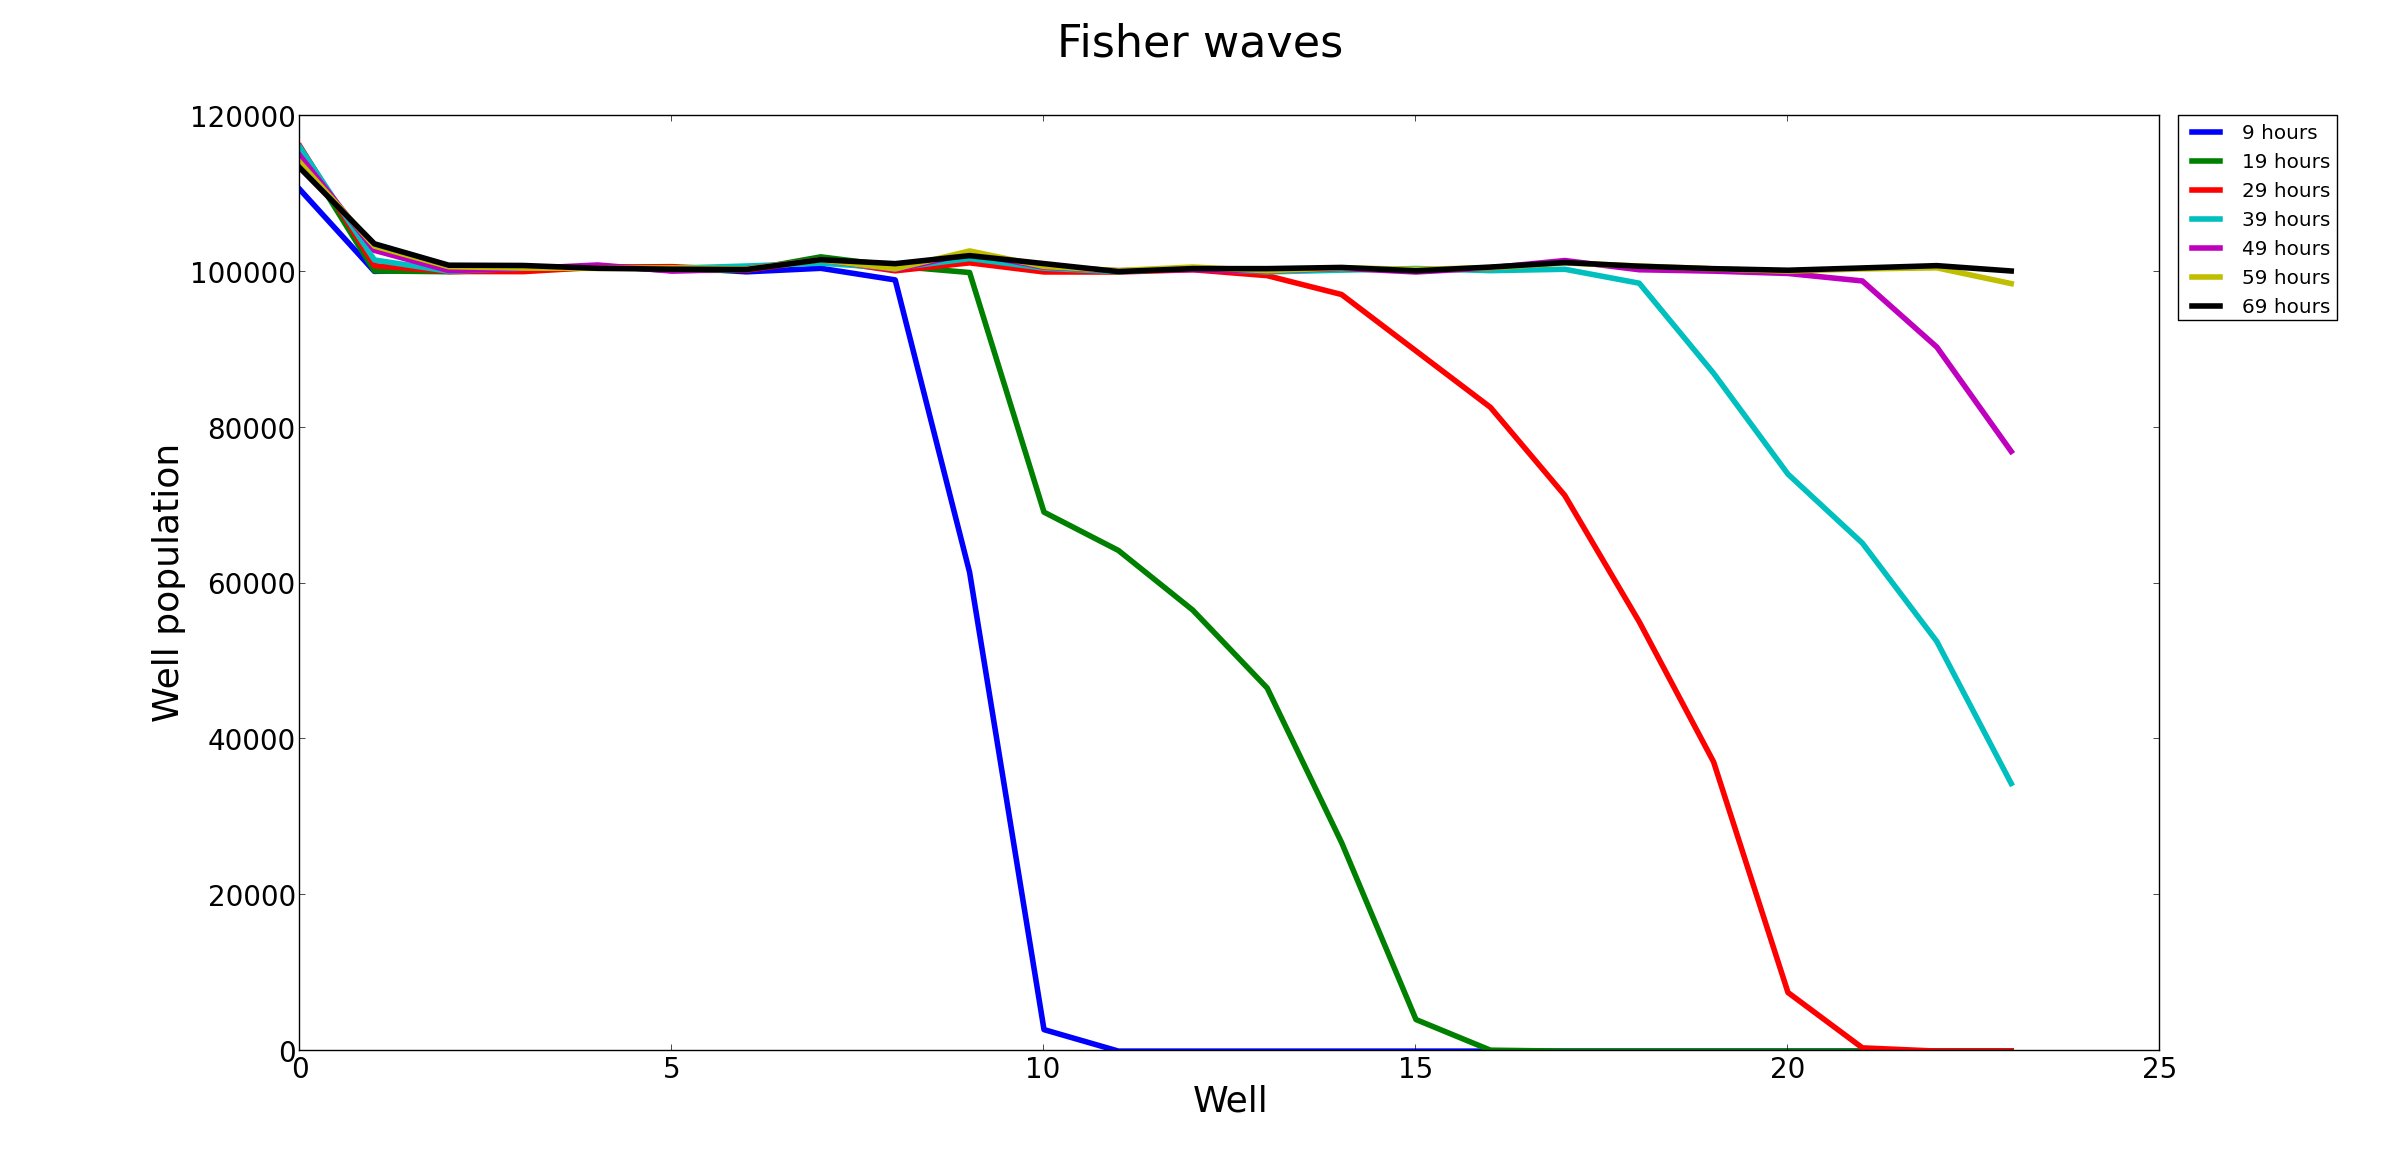
\includegraphics[width=0.95\linewidth]{waveprofiles}
\caption{Snapshots of the population at various times. We can see some bottleneck around well 10 where we were waiting for a mutation to occur.}
\label{fig:waveprofiles}
\end{figure}
 


 
 
 
% 
% 
%  \begin{figure}
%   \centering
%   \includegraphics[width=0.6\linewidth]{}
% \caption{}
% \label{fig:}
% \end{figure}
%  
%  
%  
%  
 
 
% 
% \begin{figure}[h!]
%  \begin{subfigure}{0.49\textwidth}
%   \centering
%   \includegraphics[width=0.99\linewidth]{}
%   \caption{}
%  \end{subfigure}
%  \begin{subfigure}{0.49\textwidth}
%    \centering
%   \includegraphics[width=0.99\linewidth]{}
%   \caption{}
%  \end{subfigure}
%  \caption{}
% \label{fig:expGrowthCurves} 
% \end{figure}
% 

 
 

 
 
% 
% 
% \begin{figure}[h!]
%   \centering
%   \includegraphics[width=0.6\linewidth]{sim_vs_exp_WellMixed_SingleWell}
% \caption{Comparing single-well growth curves from simulation and experiment. 
% Black: scaled experimental growth curve; orange: full stochastic simulation; purple: orange curve with time re-scaled by a factor of 2.
% Good match between simulation and experiment in the well-mixed case.}
% \label{fig:singleWell_simExp}
% \end{figure}
% 
% 
% 



% 
% \begin{figure}[h!]
%  \begin{subfigure}{0.49\textwidth}
%   \centering
%   \includegraphics[width=0.99\linewidth]{ODEs}
%   \caption{}
%  \end{subfigure}
%  \begin{subfigure}{0.49\textwidth}
%    \centering
%   \includegraphics[width=0.99\linewidth]{ODEs_2}
%   \caption{}
%  \end{subfigure}
%  \caption{}
% \label{fig:} 
% \end{figure}




% 
% \begin{figure}
%   \centering
%   \includegraphics[width=0.6\linewidth]{AB}
% \caption{}
% \label{fig:}
% \end{figure}
% 
% 







\end{document}
